\section{Exclusive Debug tools}\label{exclusive-debug-tools}

\begin{quote}
Some debugging tools for WebGL development are listed here.
\end{quote}

\href{http://www.realtimerendering.com/blog/webgl-debugging-and-profiling-tools/}{Another
post}

\subsection{WebGL Insights}\label{webgl-insights}

\href{https://github.com/3Dparallax/insight}{Home}

This tool looks very powerful and mature. Look at the features:

\begin{itemize}
\tightlist
\item
  Chrome Extension embedded in the Chrome DevTools panel
\item
  Overdraw Inspector
\item
  Mipmap Inspector
\item
  Depth Inspector
\item
  Call Stack Timeline and Statistics
\item
  Program Usage Count
\item
  Duplicate Program Usage Detector
\item
  Program Viewer
\item
  Frame Control
\item
  State Variable Editor
\item
  Resource Viewer
\end{itemize}

One screen-shot:

\begin{figure}[htbp]
\centering
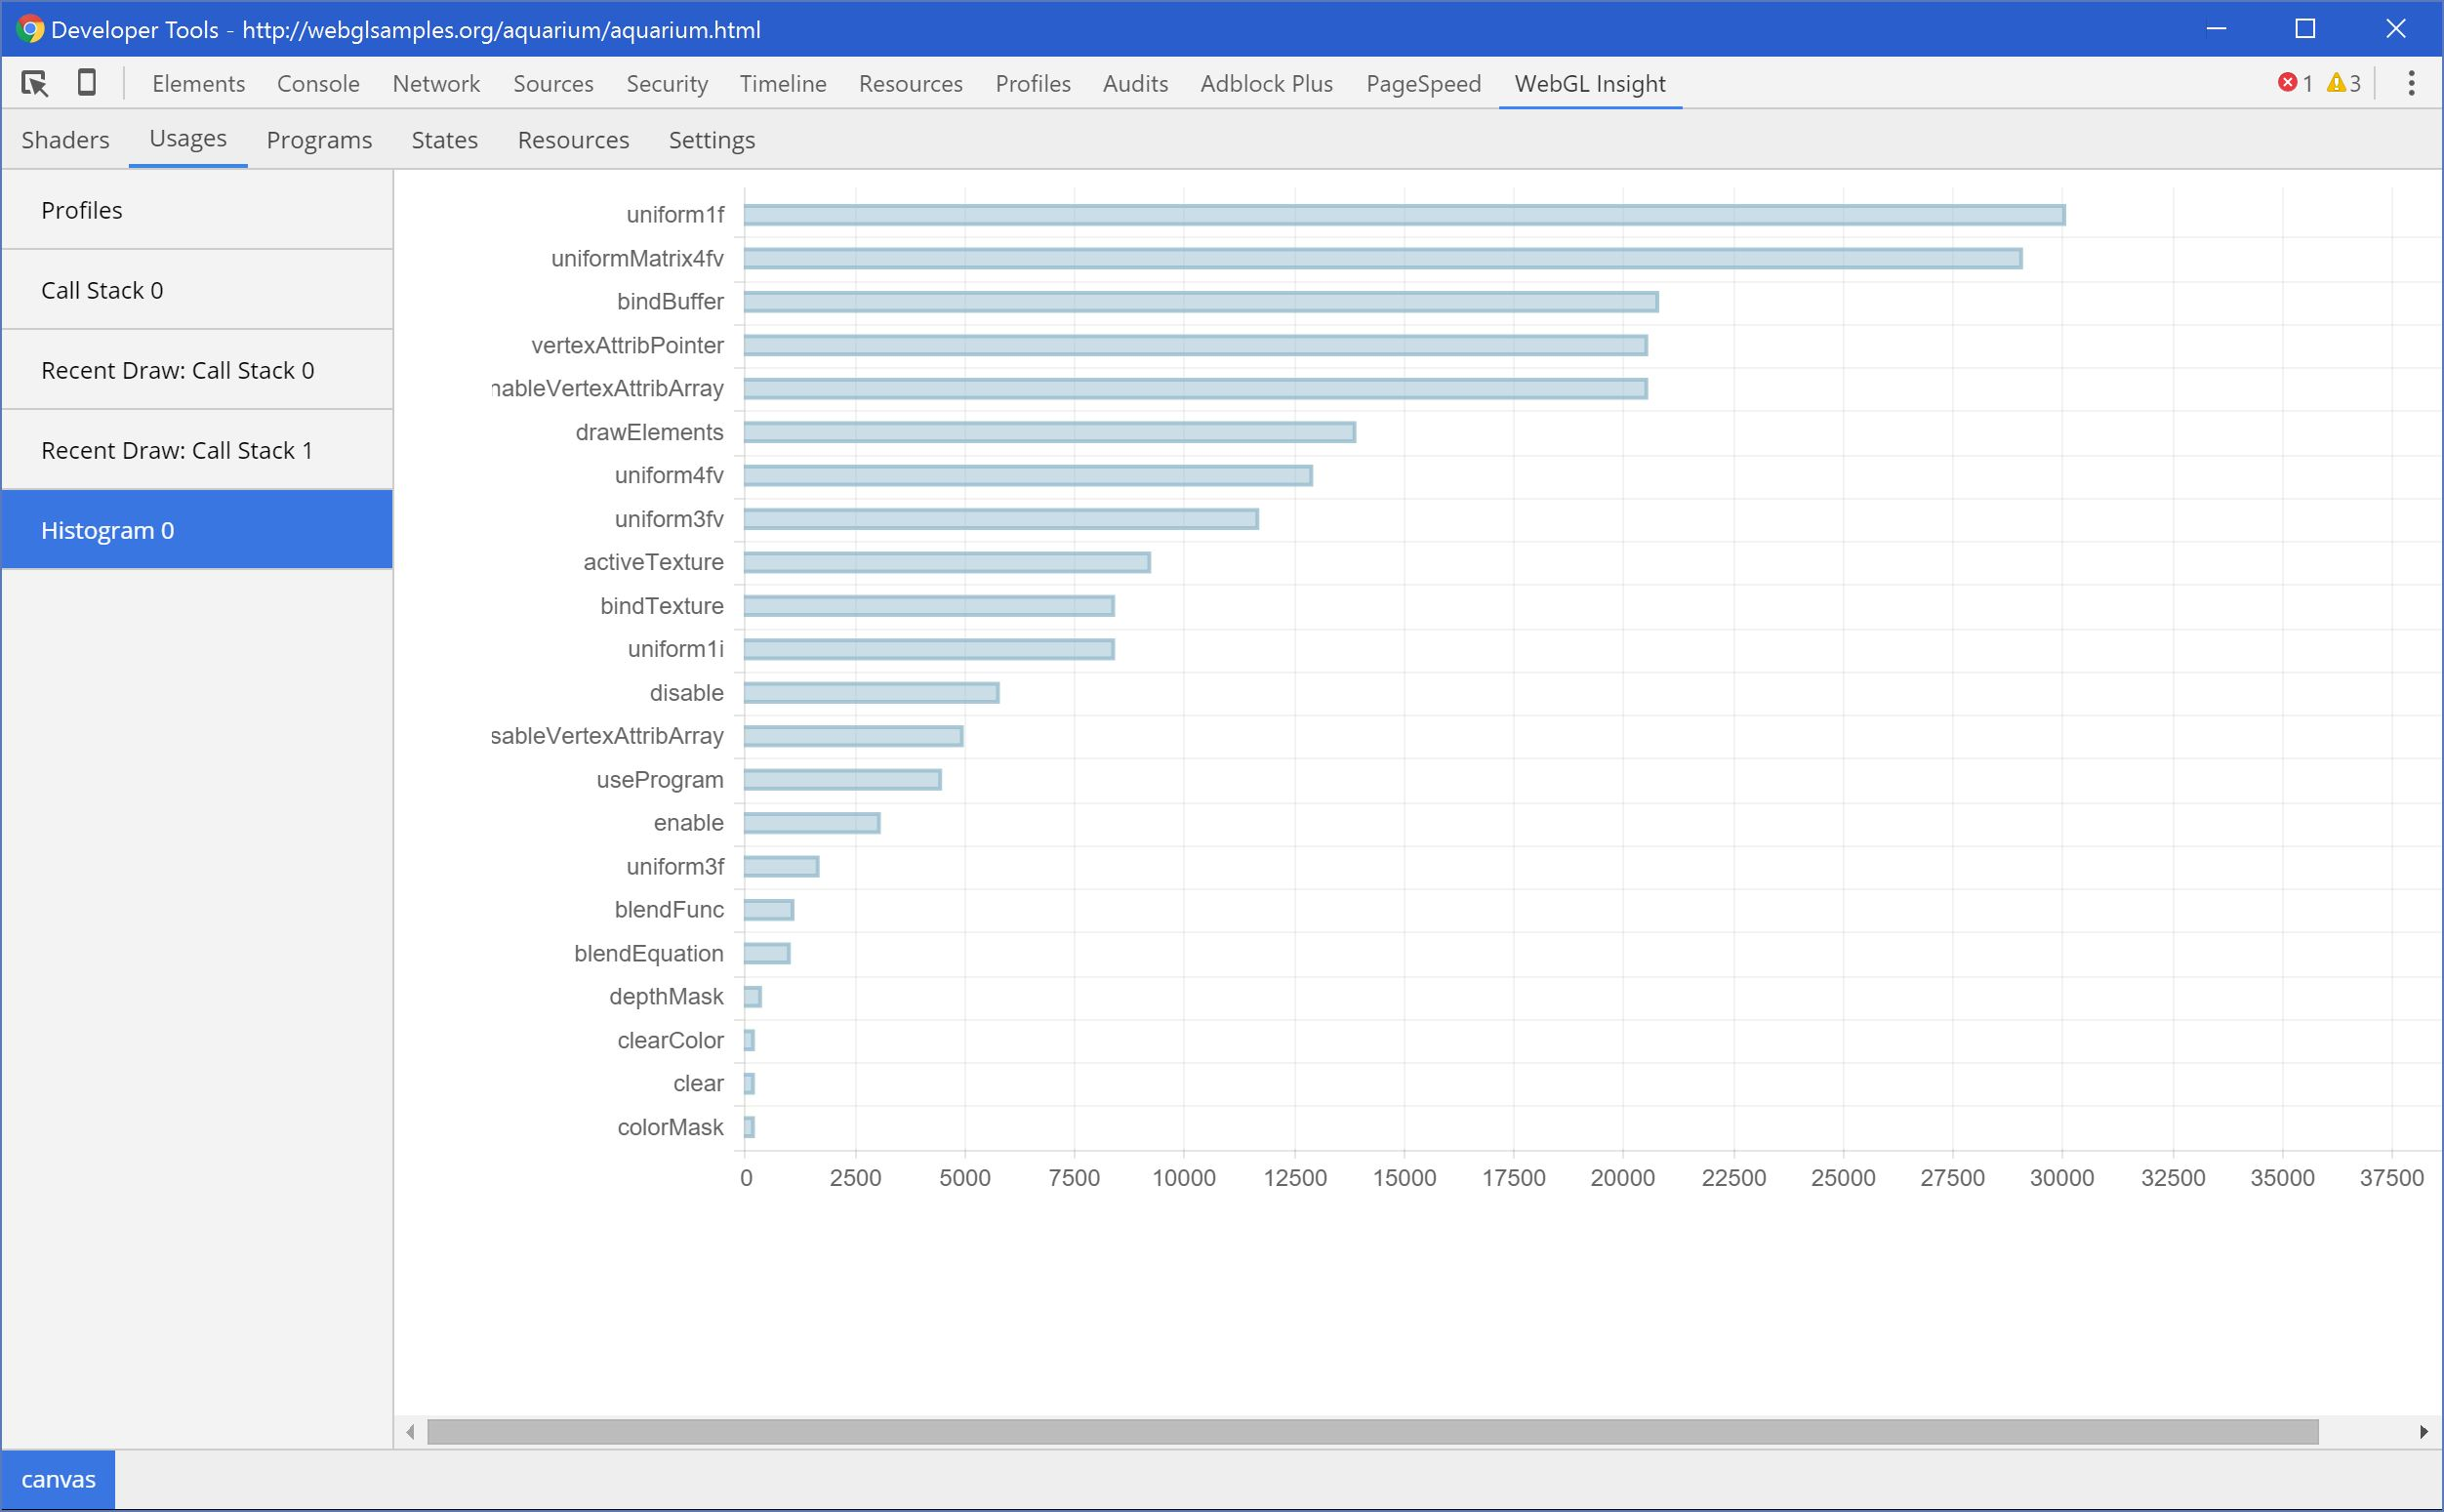
\includegraphics{insight.jpeg}
\caption{}
\end{figure}

\subsection{WebGL-Inspector}\label{webgl-inspector}

\href{https://benvanik.github.com/WebGL-Inspector/}{Home}

Features

\begin{itemize}
\tightlist
\item
  Extension for injecting into pages
\item
  Embed in an existing application with a single script include
\item
  Capture entire GL frames
\item
  Annotated call log with stepping/resource navigation and redundant
  call warnings
\item
  Pixel history - see all draw calls that contributed to a pixel +
  blending information
\item
  GL state display
\item
  Resource browsers for textures, buffers, and programs
\end{itemize}

\href{http://benvanik.github.io/WebGL-Inspector/samples/lesson05/embedded.html}{Demo}

\begin{figure}[htbp]
\centering
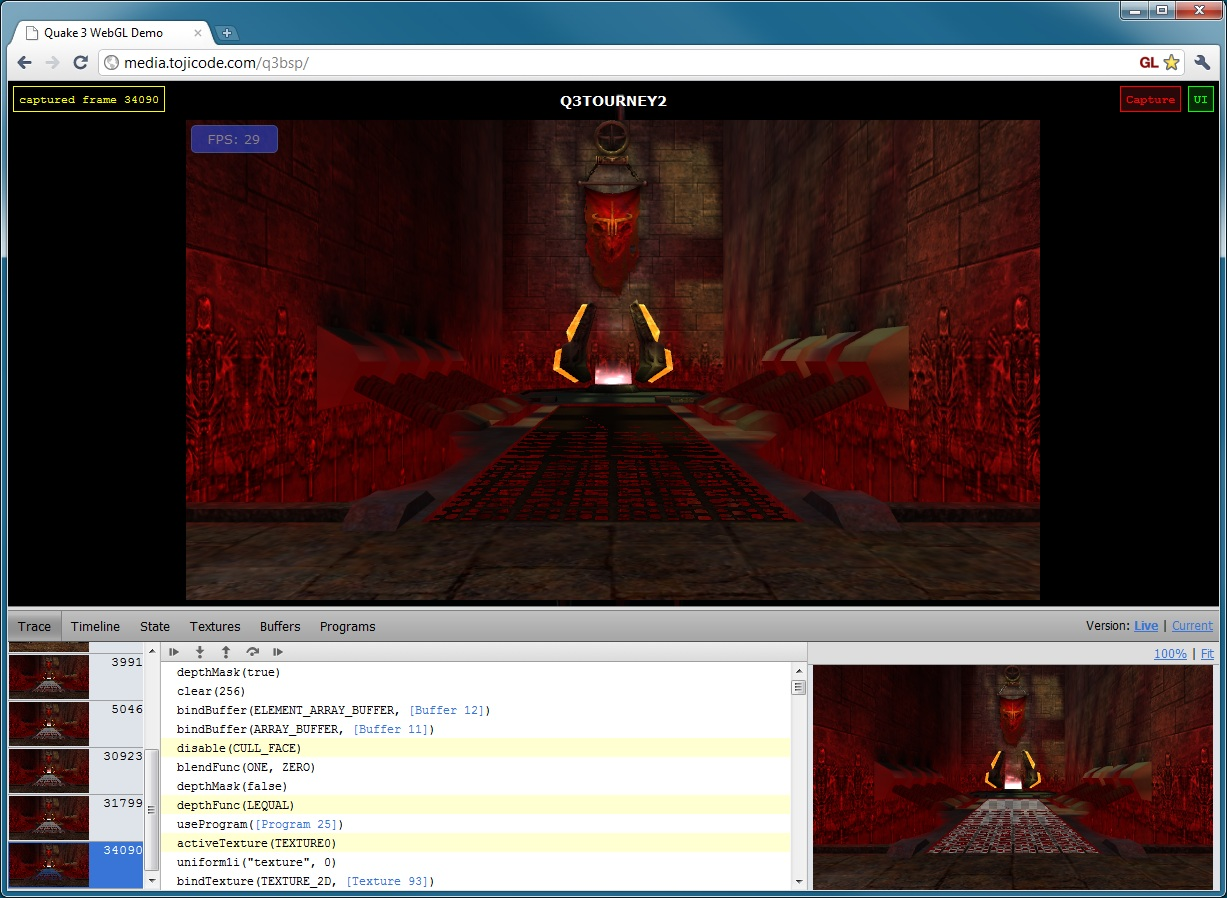
\includegraphics{inspector.jpg}
\caption{}
\end{figure}

This is a very convenient debugger, it can be useful when you
application's logic is wrong (compared to our analyzer's target -- the
syntax and API is wrong).

\subsection{webgl-debug.js}\label{webgl-debug.js}

\begin{itemize}
\tightlist
\item
  \href{https://github.com/KhronosGroup/WebGLDeveloperTools}{Repo}
\item
  \href{https://www.khronos.org/webgl/wiki/Debugging}{Home}
\end{itemize}

It will wrap the \texttt{WebGLRenderingContext} with a debugging
wrapper, which will make any GL errors show up in the JavaScript console
of browser.

Also, we can log function calls with by passing a logger in the above
mentioned wrapper.

It provides
\href{https://github.com/KhronosGroup/WebGLDeveloperTools/blob/master/src/debug/debug-sample.html}{a
sample}.

\subsection{WebGL Linter}\label{webgl-linter}

\href{https://github.com/CharlesLillo/WebGL_Linter}{Repo}

This is a discontinued and very primitive project -- but the idea is
there.
